\documentclass{article}

\usepackage{textcomp}
\usepackage{tikz}
\usepackage{amsmath}
\usepackage[hyphens]{url}
\usepackage{hyperref}
\usepackage[utf8]{inputenc}
\usepackage{relsize}
\usepackage{ifthen}
\usepackage{xstring}

\newcommand{\crel}{
	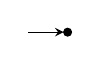
\begin{tikzpicture}[baseline={([yshift=-.8ex]current bounding box.center)}]
		\draw [->, >=stealth] (0,0) -- (0.45,0); 
		\draw [fill] (0.5,0) circle (0.05);
	\end{tikzpicture}
}

\newcommand{\rrel}{
	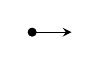
\begin{tikzpicture}[baseline={([yshift=-.8ex]current bounding box.center)}]
		\draw [fill] (0,0) circle (0.05);
		\draw [->, >=stealth] (0.05,0) -- (0.5,0);
	\end{tikzpicture}
}

\newcommand{\mrel}{
	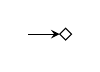
\begin{tikzpicture}[baseline={([yshift=-.8ex]current bounding box.center)}]
		\draw [->, >=stealth] (0,0) -- (0.4,0);
		\draw (0.4,0) -- (0.475,0.075) -- (0.55,0) -- (0.475,-0.075) -- cycle;
	\end{tikzpicture}
}

\newcommand{\irel}{
	\begin{tikzpicture}[baseline={([yshift=-.8ex]current bounding box.center)}]
		\draw [->, >=stealth] (0,0) -- (0.4,0);
		\draw (0.41,0) -- (0.55,0);
		\draw (0.48,-0.07) -- (0.48, 0.07); 
	\end{tikzpicture}
}

\newcommand{\erel}{
	\begin{tikzpicture}[baseline={([yshift=-.8ex]current bounding box.center)}]
		\draw [->, >=stealth] (0,0) -- (0.4,0);
		\draw (0.41,0) -- (0.55,0);
		\draw (0.48, 0.05) circle (0.02);
		\draw (0.48, -0.05) circle (0.02); 
	\end{tikzpicture}
}


\title{DCR/TEE \\
\large Working subtitle in a trusted execution environment}
\author{Mikkel Gaub \and Malthe Ettrup Kirkbro \and Mads Frederik Madsen}

% Allow line break at ',' in math mode:
\makeatletter
\def\old@comma{,}
\catcode`\,=13
\def,{%
  \ifmmode%
    \old@comma\discretionary{}{}{}%
  \else%
    \old@comma%
  \fi%
}
\makeatother

% C++ command
\newcommand\cpp{C\nolinebreak[4]\hspace{-.05em}\raisebox{.4ex}{\relsize{-1}{\textbf{++}}}}

\begin{document}
\sloppy

\begin{titlepage}
	\maketitle
	\pagenumbering{gobble}

	\vspace{\fill}
	\begin{abstract}
		In this thesis the security and optimization options provided by recent advances in trusted execution environments (TEE), specifically Intel Secure Guard Extensions (SGX), are explored in relation to the known problem of decentralized replication.
		An algorithm, and the implementation of that algorithm, for running decentralized Dynamic Condition Response (DCR) graphs is used as the example of a system requiring decentralized replication.
		Lastly a description of what it would require to transform the developed system to be able to handle general smart contracts is given.
	\end{abstract}
\end{titlepage}

\clearpage
\pagenumbering{arabic}

\tableofcontents

\newpage

\section{Introduction}

	Replication of data in decentralized and arbitrarily large networks, is not a new problem, and is a core challenge for many distributed systems.
	Existing solutions to this problem are expensive, in the sense that they require a large number of messages to be exchanged and slow in that they provide a low degree of concurrency.
	The tools afforded to us by recent technological advances, provide strong guarantees and advantages which could potentially be leveraged to improve existing solutions to the problem of decentralized replication.
	Trusted execution environments, such as Intel Software Guard Extensions (SGX), provides a verifiable trusted subsystem to each participant, which is especially interesting in a decentralized system of mutually untrusting nodes.

	In a time where collaboration between companies, small and large, occurs daily across vast physical distances, a trusted means of coordination is key.
	An example of this are Dynamic Condition Response (DCR) graphs, which is a declarative workflow management system.
	A core neccesity of DCR is the agreement of all parties on what has transpired in the workflow and what the state of the workflow is at any given point.
	Depending on how a specific DCR graph is constructed, it can potentially allow for a very high degree of concurrency, as each node in a DCR graph can only affect the states of neighbouring nodes.
	DCR graphs will serve as the subject of the replication for this project.

	The goal is therefore a decentralized DCR engine distributed among \textit{p} participants, which for a DCR graph, \textit{g}, ensures that all \textit{p} adhere to the semantics of \textit{g}.
	Any \textit{p} should at any time be allowed to request a state change, provided that \textit{p} is verifiably allowed to perform this state change and that this state change is not incompatible with any simultaneous state change.
	A state change is only required to be propogated to the nodes which that state change matters to, with respect to \textit{g}.
	Collection of a global state, \textit{s}, should be possible at any time, by any \textit{p}.
	A global state should always be compatible with any other global state for the same graph.

	\subsection{Problem}

	The solution is outlined by the following summarized requirements.
	The system must:
	\begin{itemize}
		\item Support the replication of a decentralized DCR graph, while maintaining a high degree of concurrency as permitted by DCR.
		\item Achieve consensus on the state of a decentralized DCR graph in less than a quadratic number of messages.
		\item Function in a highly malicious environment, where the only guarantees are those based on strong cryptographic security.
	\end{itemize}

	\noindent The contributions of this thesis are as follows:
	\begin{itemize}
		\item The design and implementation of the solution outlined above.
		\item A detailed description of the expansion of the implementation to support arbitrary smart contracts rather than DCR graphs.
		\item An argument for the introduction of trusted execution environments reducing byzantine faults to crashes, in any distributed system.
	\end{itemize}

\section{Related works}

	An existing platform which partially provides a solution to the goal of this project is Ethereum \cite{_ethereum_2018}.
	Ethereum is a distributed computing platform based on blockchain technologies, which does, however, also feature a currency, making computations disproportionately expensive, both monetarily and computationally due to the large amounts of computations required by proof-of-work based blockchains.
	Even though SGX is a new technology, it has already been proposed to solve several issues in the blockchain concept. 
	SGX has been used as an intermediate for faster consensus about transactions in \cite{gopinath_nirmala_improving_2017}, however it still relies on the underlying blockchain to prevent double-spending.

	In \cite{liu_scalable_2016} SGX has been utilized to implement a new Byzantine fault tolerance (BFT) consensus algorithm, called \textit{FastBFT}, which solves some of the scalability issues of blockchains.
	This is done by using the \textit{strawman design} where a request is sent to a node, the \textit{primary}, who prepares a vote by distributing parts of a secret to all nodes.
	The secret can be reconstructed given enough parts and then compared to the hash of the secret which is common knowledge.
	This means that consensus can be achieved in only $O(n)$ messages, rather than the $O(n^2)$ messages achieved by other algorithms.
	The reason that Intel SGX is needed for this algorithm is that the primary, who distributes the secrets, can fake being any node as he has all parts of the secret.
	Trusted Execution Environments (TEE) as introduced by Intel SGX, means that these secrets can be computed and distributed without the primary every having access to them.
	A further issue with the strawman design, is that the primary can change the orders of requests, thereby equivocate which request is being voted on.
	This is once again solved by Intel SGX, by numbering requests with a trusted counter that can only be incremented.

	In particular, the Hyperledger Sawtooth \cite{dhillon_hyperledger_2017} project is interesting as it is closely related to the goals of our project.
	Hyperledger Sawtooth is an ongoing blockchain project, which replaces the need for mining by using a consensus algorithm called Proof of Elapsed Time (PoET).
	In PoET a number of nodes who choose to participate as validators each create a timer using Intel SGX.
	This timer is different per validator and contains a timestamp some time in the future, with a degree of randomness.
	A validator can also check that a timer is valid, using Intel SGX, and also whether or not that timer has expired.
	The first validator to distribute a valid and expired timer to the rest of the validators, is elected leader for the current round of decision-making.	
	This is a strong indicator that Intel SGX can be used for efficiently attaining consensus.

	\subsection{Definitions}
	\noindent
	Workflow: $G=(V,E)$ \\
	Activities: $V=\{v_1,\ \dots, v_n\}$ \\
	Activity States: $S=\{s_1,\ \dots, s_n\}$, where $s_i \subseteq \{Executed, Pending, Included\}$ corresponding to $V_i$.\\
	Relation: $R=($condition, response, milestone, include, exclude$)$, $e=(v_x, v_y, r_i)$, $E=\{e_1,\ \dots, e_m\}$\\
	Processes: $P =\{p_1,\ \dots, p_o\}$.\\
	History, $H_p(t)$: Sequence of activity executions up to, and at time $t$, as perceived by given process.\\
	Execution: $(v_i, t, p)$, where $v_i$ is the activity executed at time $t$, executed by process $p$.\\
	Dependant activities: An activity, $v_1$ is said to be dependent on another activity, $v_2$, when the DCR rules allowing $v_1$ to be executed, depends on the state of $v_2$. \\
	% Processor: $C$ is said to own a number of specific processes. Any process can only be owned by a single processor. \\
	% Activity responsibility: ... \\

	\subsection{Requirements}
	\begin{description}
		\item[Consensus]:
			\begin{description}
				\item[Termination] Eventually each correct process sets its decision value (single activity state)
				\item[Partial agreement] % Decision vector = activity state
								Bottom is allowed as substitute for any activity state, unless that activity is owned by process or dependent on one such process. % Hvad er agreement
				\item[Integrity] If $p_i$ is correct, then all correct processes decide on $v_i$, or $\bot$ as the i'th component of their vector. % Omformuler. Kan ikke genbruge i på den her måde
			\end{description}
		% \item[Concurrency]: DCR-rules for concurrency (only independent activities can be concurrent) (Tie-breaking). Nødvendig? Argumentér hvorfor Agreement + integrity giver concurrency løsning
		\item[Correctness]: Any state transition must be permitted by DCR logic or they will be rejected by correct nodes.
		\item[Non-repudiation]: $v_i$ must be provably proposed by $p_i$, within the bounds specified by any applied cryptography.
		% \item[Co-non-repudiation?]:
	\end{description}

\section{DCR}

A DCR graph is a representation of a workflow, made up of one or more events with a number of relations between them. 

		\subsection{Event State}
		The events in a DCR graph have three binary attributes: included, executed and pending. 
		Furthermore an event can have role and actor specific execution rights.
		This is an event: \ev{A}

			\subsubsection*{Executed attribute}
			If an events executed attribute is false executing the event will set its executed attribute to true.
			Executing an already executed event will have no effect on the executed attribute.
			The executed attribute is shown as a tick mark: \ev[101]{A}

			\subsubsection*{Pending attribute}
			If any event in a workflow has a pending attribute that is true and the event is included, the workflow is in an unfinished state.
			Every time an event is executed its pending attribute is set to false.
			This means that setting the pending attribute of an included event to true is specifying that this event must be executed or excluded at some point to leave the workflow in a finished state.
			The pending attribute is shown as an exclamation point: \ev[011]{A}

			\subsubsection*{Included attribute}
			If the include attribute of an event is true, the event is included and it can be executed. 
			If the attribute is false, the event is excluded and can no longer be executed.
			The included attribute is denoted by the outline of the event: \ev{A} when included and \ev[000]{A} when excluded.

		\subsection{Relations}
		There are five types of relations which define different types of relationships between events in a workflow. 
		All relations can be said to originate from an event and targeting an event.
		The origin and the target of a relation can be the same event.
		The five can be divided into two categories:

		\begin{description}
			\item[Effects] which are relations that propagate an execution to other events, in the sense that they change the state of the targeted event. 
			If an effect originating from an event, \texttt{A}, is targeting an event, \texttt{B}, then \texttt{A} is said to be the effecting event on the effected event \texttt{B}. % affected?
			These are the \emph{response}, \emph{include} and \emph{exclude} relations. 
			\item[Constraint] which are relations that exclusively affect whether or not the targeted event can be executed. 
			If a constraint originating from an event, \texttt{A}, is targeting an event, \texttt{B}, then \texttt{A} is said to be the constraining event on the constrained event \texttt{B}.
			These are the \emph{condition} and \emph{milestone} relations. 
		\end{description}

			\subsubsection*{Condition relation}
			If there is a condition relation from event \texttt{A} to event \texttt{B}, then \texttt{B} can only be executed if \texttt{A}'s executed attribute is true or \texttt{A} is excluded.
			This described situation can be shown as: $\ev{A} \crel \ev{B}$

			\subsubsection*{Response relation}
			If there is a response relation from event \texttt{A} to event \texttt{B}, then \texttt{B}'s pending attribute will be set to true every time \texttt{A} is executed.
			This described situation can be shown as: $\ev{A} \crel \ev{B}$

			\subsubsection*{Include relation}
			If there is an include relation from event \texttt{A} to event \texttt{B}, then \texttt{B}'s included attribute will be set to true every time \texttt{A} is executed.
			This described situation can be shown as: $\ev{A} \crel \ev{B}$

			\subsubsection*{Exclude relation}
			If there is an exclude relation from event \texttt{A} to event \texttt{B}, then \texttt{B}'s included attribute will be set to false every time \texttt{A} is executed.
			This described situation can be shown as: $\ev{A} \crel \ev{B}$

			\subsubsection*{Milestone relation}
			If there is a milestone relation from event \texttt{A} to event \texttt{B}, then \texttt{B} can only be executed if \texttt{A}'s pending attribute is false or \texttt{A}'s included attribute is false.
			This described situation can be shown as: $\ev{A} \crel \ev{B}$

		\subsection{Enabledness}

		Since the properties of DCR graphs described so far, all affect whether or not a given event can be executed or not, we use the notion of enabledness to describe the sum of these properties.
		An event which can be executed, meaning it is included and any milestones or conditions targeting it are rendered invalid by the state of the relevant events, it is said to be enabled.
		If an event cannot be executed, due to the inverse of the aforementioned prerequisites, it is said to be disabled.
		If an event changes from being enabled to disabled or from disabled to enabled, its enabledness is said to have changed.

		\subsection{Concurrency}
		Concurrency can be achieved to a degree in a given DCR graph, depending on the exact construction of that graph, due to the fact that event executions have a limited reach with regards to what states they can modify. 
		Events which can be executed concurrently are said to be independent of one another.
		For example, given the graph: $\ev{A} \erel \ev{B}, \ev{C} \irel \ev{B}$, \texttt{A} and \texttt{C} are not independent, as they both have an effect on the state of \texttt{B}.
		Whereas in the graph: $\ev{A} \crel \ev{B}, \ev{C} \crel \ev{B}$ \texttt{A} and \texttt{C} are concurrent, as they have no effect on each other or on a shared event.

			\subsubsection{Event Independence}
			There are two types of independence analyses relevant for this paper:
			\begin{description}
				\item[Static independence] means that for two event and the state of them, are they independent.
				\item[Dynamic independence] means that for two events, are they independent in every state they could be in. This problem belongs to NP and an approximation will have to be used instead.
			\end{description}

\section{Intel SGX}

	Intel SGX is a TEE technology which allows users to define protected areas of memory, so called \textit{enclaves}.
	Intel guarantees \cite{intel_sgx} that any code run and data loaded in the TEE is protected from access by any process running outside of the enclave.
	More specifically, the guarantees encompass \textit{confidentiality}, i.e. no other process can read the data in the enclave, and \textit{integrity}, i.e. no other process can modify the data in the enclave. 
	If the enclave contains secrets which the user wishes to keep, but still does not want to trust external processes with, the enclave can be sealed on disk, essentially encrypting it for later use.
	This means that data can be stored and processed securely, with its security guaranteed by Intel, if done properly.
	An additional feature of Intel SGX is that the result of any code run using Intel SGX can be verified by other users, given the code and the output.

	This is all made possible by unique keys generated during manufacturing and permanently stored inside the fuse array of the processor.
	Some of these keys are known by Intel for the system to be recognized when contacting Intel servers.

	In short, the major innovation in Intel SGX is the option of running hardware secured software, which enables tamper proof messages, where the sender can be verified as being a correct process.
	This eases some of the inherent problems in consensus, as seen in \cite{liu_scalable_2016} and \cite{dhillon_hyperledger_2017}.

		\subsection{Enclave}
		\label{subsec:enclave}
		What allows SGX enabled CPUs to provide these strong guarantees builds on the following two hardware details:
		\begin{description}
		\item [Processor Reserved Memory (PRM)] is a sequential block of memory reserved for SGX, inaccessible from untrusted software and even hardware.
		\item [Enclave mode] is a mode under which a logical processor gains access to the PRM.
		\end{description}
		Using these hardware facilities SGX defines the concept of an enclave.
		An enclave is, as its name suggests, a software module isolated completely from the rest of the system.
		Its memory is located solely in PRM, preventing access by other processes and enclaves running on the system. 
		The PRM is protected from non-enclave processes by enclave mode. 
		When a process is not in enclave mode and tries to access the PRM, the memory access is denied \cite{costan_intel_2016}.      
		The PRM of an enclave process is protected from accesses by other processes in enclave mode by the SGX Enclave Control Structure (SECS). 
		The SECS holds meta data about the enclave processes, and among this is a virtual-to-physical memory mapping called the Enclave Page Cache (EPC). 
		Through the EPC an enclave's access to physical PRM is restricted to what has been allocated for the enclave-process \cite{costan_intel_2016}.

		While SGX provides powerful guarantees trough its enclave concept, it does not guarantee software correctness and will not protect against flawed software.
		Instead SGX encourages developers to isolate a minimal piece of their software, the Trusted Computing Base (TCB), in a trusted enclave environment, and keep the remainder as traditional system processes \cite{intel_sgx_guide}.
		By minimizing the size of the TCB, and thus the amount of code one must trust, common security principles indicate that the chance of security flaws decreases \cite{intel_sgx_guide}.

		In order for an isolated enclave to be useful, communication between trusted and untrusted software is enabled through \textit{enclave calls} (ECALL) and \textit{out calls} (OCALL).
		This interface must be defined at compile-time, specifying an API of ECALLs for the enclave as well as any untrusted services needed as OCALLs, in a \textit{EDL}-file \cite{intel_sgx_guide}.

		When built, an enclave module is a plain binary on the untrusted file system.
		As an enclave under such circumstances would be vulnerable to tampering before initialization, SGX enforces a strict signature policy.
		An enclave must include an \textit{Enclave Signature} containing \textbf{(a)} a hash of the code and initialization data of the enclave, \textbf{(b)} the author's public key and \textbf{(c)} an enclave version/product number.
		During enclave initialization a hardware check is performed, ensuring the Enclave Signature matches the enclave binary loaded from the file system.

		Another powerful tool of an SGX enclave is the ability to read from and write data to an untrusted storage medium while ensuring confidentiality of its contents.
		Such capabilities are needed as the PRM is volatile and will not persist after shutdown.
		In SGX this process is known as \textit{sealing}.
		Sealing allows encryption and decryption using a \textit{Seal Key}, which is confidential to the Enclave Signature.

		\subsection{Attestation}
		\label{subsec:attestation}
		Attestation, within the Intel SGX platform, is the action of verifying the existence of specific enclaves.
		The applications of this are two-fold, in the case where there are multiple enclaves running locally on the same CPU and in the case where enclaves need to communicate to enclaves running on external CPUs.
		These two situations are handled by two different processes, aptly named local and remote attestation.
  
		Local attestation builds on a secret fused into the CPU.
		An enclave can use an SGX instruction to generate a report uniquely identifying the enclave.
		This report is MACed with a key derived from the fused secret and enclave identifier.
		It is not possible to fake such a MACed report, as the MACing happens in hardware components that ensure that the report corresponds to the caller enclave.
		The fused secret is not directly accessible by software components, but can only be used by certain hardware instructions that protect against malicious use.
		An attestation challenger will ask for a MACed report from the client enclave, and after receiving it derive the same key to verify the MAC.
		Because a report can only be created by the enclave it describes, the challenger can be certain of which enclave the client is running if the MAC is valid.
		To prevent replays the MACed report is allowed to contain a block of arbitrary data, in which the challenger can require a nonce.

		Remote attestations build on the same concept of a report, but as challenger and client are now on different CPUs, they no longer hold the same fused secret.
		Instead remote attestation relies on the group signature scheme Enhanced Privacy ID (EPID) and a third party issuer.
		Each SGX enabled CPU is granted an EPID Member Private Key by the third party issuer some time after manufacturing.
		Like the fused secret, this private key is not directly accessible to an enclave.
		Under the EPID scheme, all issuer generated private keys share the same public key (EPID Group Public Key).
		When remote attestation takes place, the client enclave generates a report and attests locally with the Quoting Enclave (QE).
		The QE, now convinced of the client enclave's identify, strips the MAC off the report and instead signs it with the EPID Member Private Key, which the QE has special privileges to access\footnote{Enclaves signed by Intel have special privileges throughout SGX. This allows SGX to implement complicated SGX instructions in software.}.
		The remote challenger can verify the signed report with the EPID Group Public Key and be sure that \textbf{(a)} the report is signed by an EPID Member Private Key, \textbf{(b)} EPID Member Private Keys are granted secret to QEs, and \textbf{(c)} QEs will not sign false reports.

		\subsection{Monotonic counters}
		One of the functions provided by Intel SGX, which is especially relevant for this project, is the access to \textit{trusted monotonic counters}.
		As indicated by the name, monotonic counters are integer counters, that can only be incremented.
		They are implemented as a block of non-volatile memory accessible only through SGX instructions, protecting against replay attacks.

		\subsection{Transforming byzantine faults to crashes}
		We conjecture that the correct use of Intel SGX can transform all byzantine faults in a distributed system with unreliable channels to crashes.
		To be precise, we define a byzantine fault to be "a fault presenting different symptoms to different observers" \cite{driscoll_byzantine_2003}, and an unreliable channel to be a channel in which messages can be lost, delayed, duplicated and reordered.
		We assume that processes that exhibit byzantine faults will not be able to guess the secrets of a byzantine-resistant subsystem.
		We will show that Intel SGX can remove these faults in three steps: 
		First we will show that Intel SGX is in itself a byzantine-resistant subsystem, i.e. a subsystem that cannot exhibit byzantine faults.
		Then we will show that sending messages from a byzantine-resistant subsystem through a component exhibiting byzantine faults (such as the host OS) is equivalent to sending a message over an unreliable channel if the message is integrity-protected.
		And lastly, we will show that using these two properties, any distributed system can be transformed from exhibiting byzantine faults to exhibiting at most crashes, given that all messages can be verified to be produced by a byzantine-resistant subsystem.

		Intel SGX has guaranteed \textit{integrity} by Intel \cite{intel_sgx}.
		That is, enclave memory written by an Intel SGX process is guaranteed tamper proof.
		Intel achieves this using two mechanisms: Processor Reserved Memory (PRM) and cryptographic integrity checks.
		PRM prevents access to enclave memory at hardware-level, which means that only the appropriate Intel SGX process is able to access the memory, see section \ref{subsec:enclave} for a detailed explanation.
		However, this does not alone prevent byzantine faults, as byzantine faults are not only produced by other processes.
		For instance, the infamous Single Upset Event (also knowns as cosmic ray bit flips) \cite{normand_single_1996}, is a byzantine error where bits in memory are flipped due to background radiation. 
		Intel SGX protects against such hardware errors by using cryptographic integrity checks \cite{gueron_memory_2016}.
		When loading enclave memory, Intel SGX's Memory Encryption Engine (MEE) decrypts the memory, and then performs an integrity check on the loaded memory.
		If the integrity check does not pass, the processor drops the memory, and eventually locks itself for further operations (the \textit{drop-and-lock policy}), requiring a physical reset before new operations can be completed \cite{jang_sgx-bomb_2017}.

		In short, the integrity checks is implemented as a Merkle-Tree of Message Authentication Codes (MACs), with the root node of the tree stored on processor-internal memory \cite{jang_sgx-bomb_2017}. 
		Under the assumption that AES128 is a random permutation, this method provides the guarantee that an active adversary with the capability of observing the MACs has a negligible probability of forgery \cite{gueron_memory_2016}.

		A practical example of the effectiveness of this integrity check is the \textit{SGX bomb} attack \cite{jang_sgx-bomb_2017}. 
		The SGX bomb, is a denial-of-service attack on Intel SGX. 
		It utilises a Row hammer attack to flip arbitrary bits in the EPC, thus triggering the drop-and-lock policy when memory is loaded.
		But this just demonstrates that even given the power to flip arbitrary enclave bits, the worst attack an adversary can mount is a processor crash.

		\begin{table}
			\centering
			\begin{tabular}{l|l}
				\textbf{Adversary action} & \textbf{Channel failure equivalence} \\\hline
				Delete $m$                  	& Losing $m$                     \\\hline
				Withhold $m$                	& Losing $m$                     \\\hline
				Resend $m$                  	& Duplicate $m$                  \\\hline
				Withhold $m$, ..., resend $m$ 	& Reorder of $m$                
			\end{tabular}
			\caption{Adversary action/Channel failure equivalency\label{tab:adversary-failure-equivalency}}
		\end{table}

		Given that Intel SGX is byzantine-resistant, we will now show that sending messages from a byzantine-resistant subsystem through a process that can exhibit byzantine faults, is equivalent to sending the message over an unreliable channel, if the message is integrity protected.
		In this terminology, an unreliable channel is a channel in which messages can be lost, delayed, duplicated and reordered.
		Given a message, a byzantine man-in-the-middle adversary can either delete it, withhold it, resend it, tamper with it or any combination thereof\footnote{Some of the combinations of actions are equivalent with just one action, for instance deleting a message and then resending is exactly equivalent of resending it -- we will not take these combinations into account}.
		From the point of view of the sender and recipient each of the adversary's methods is exactly equivalent to a channel failure as specified by table \ref{tab:adversary-failure-equivalency}.
		The only thing that the adversary can do, that has no equivalence in channel failures, is to tamper with the message.
		But if the message is integrity protected, any tampering will be evident to the recipient, and thus the recipient can discard the message. 
		Thereby the adversary tampering with a message becomes equivalent to the channel failure of losing the message. 

		In practice, the integrity protection of the message can be implemented in Intel SGX, by sharing a cryptographic key during remote attestation, and then MACing messages with this key when sending messages between enclaves. See section \ref{subsec:attestation} for more information. %Attestation is missing something about key exchange

		Given that communication between byzantine-resistant subsystems over a layer exhibiting byzantine faults is reduced to unreliable channels if the messages are integrity protected, we can now show how to reduce all byzantine failures to crashes in a system unreliable channels, if all messages can be verified to have been produced by byzantine-resistant subsystems:

		To remove byzantine faults, each process must simply run a byzantine-resistant subsystem, responsible for running the protocol.
		The subsystems must be attested, and during this attestation exchange a secret key for producing MACs.  
		All communication might have to pass through the byzantine processes, but given message integrity from the MACs, this simply reduces to unreliable channels. 
		If a process tries to participate in the protocol without such a subsystem, recipients of that process' messages will know that it was not produced by a byzantine-resistant subsystem, and can simply discard the message.

		In practice, the MACing of the message also serves as proof that it was produced by an Intel SGX process, as the MAC key was exchanged during attestation, thereby guaranteeing that the key is stored in an enclave. 



	\section{Algorithm}
	\label{sec:algorithm}
	%This section uses the following terms, which must therefore be introduced before this section:
	% - closed neighbourhood
	% - Second neighbourhood

	For any algorithm to guarantee workflow correctness of a distributed DCR graph in an asynchronous setting, the algorithm must (1) push executions to effected neighbours and (2) synchronize the executions of non-independent events.
	This section provides the reasoning behind these requirements.
	Furthermore, this section will show (3) that an execution of an event can change the state of events only in the immediate neighbourhood, and (4) that an execution can change the enabledness of events only if the events are in the closed neighbourhood of the closed neighbourhood of the executing event.  

	We will describe the algorithm under the most general case where each event is handled by a separate peer.
	For simplicity e.g. $A$ will refer to both the event and the peer responsible for it.
	% We will show that this workflow is enough to describe a general algorithm when $A$ is executed.
	% Something with events only chaining state one degree forward and thereby enabledness two degrees forward. 
	% Why?

	% Effects must push execution state (1)
	Consider the events $A$, $B$ and $C$, where $A$ has relation $AB$ to $B$, and $B$ has relation $BC$ to $C$.
	When $AB$ is an effect ($A\irel B$, $A\erel B$ or $A\rrel B$), $B$ must be informed of any execution of $A$ (1).
	To see this is the case, consider the workflow $(\{D, E, F\}, \{D\erel F, E\irel F\})$, where $D$ and $E$ has been executed.
	As $F$ is not immediately informed about executions of $D$ and $E$, an execution attempt at $F$ must query $D$ and $E$ to determine the inclusion state of $F$.
	Such a query would require an ordering of executions of $D$ and $E$, which is not generally possible in an asynchronous setting.

	% AB effects must synchronize (2)
	When an execution happens on an event with an effect to another event, some degree of synchronization must occur between a subset of peers (2).
	To see this is the case, consider the workflow $(\{D, D', E, E'\}, \{D\irel E, D\erel E', D'\erel E, D'\irel E'\})$.
	We showed executions must be propagated along effects in an asynchronous setting.
	Thus when executing $D$ and $D'$, messages $M_{D\irel E}$, $M_{D\erel E'}$, $M_{D'\erel E}$ and $M_{D'\irel E'}$ are required.
	The ordering of these messages can not generally be guaranteed in an asynchronous setting.
	To see why synchronization must occur, consider the message arrival sequence $(M_{D\irel E}, M_{D'\erel E}, M_{D'\irel E'}, M_{D\erel E'})$, resulting in an invalid workflow state where both $E$ and $E'$ are excluded.

	%Executions of events can only effect state in the immediate neighbourhood (3)
	Executions of events can only effect state in the immediate neighbourhood (3).
	When event A is executed, its \texttt{Executed} state will change, and all events that A has an effect relation to, has its appropriate state variable changed. 
	In other words, one state change propagates to state changes along effect relations. 
	However, the only state change that propagates to state changes in other events is the change of the \texttt{Executed} variable.
	And since none of the effect relations change the \texttt{Executed} variable, the state change can at most propagate to the immediate neighbourhood of the executing event.
	Notice that state change does not propagate along constraint relations, but the enabledness of events along these relations are still changed. 
	However, enabledness cannot propagate, since no state change is induced by a change in enabledness, and enabledness itself is changed only by state changes in the constraining event. 

	%Rewrite this?
	From (3) we also gain (4), that enabledness is at most changed in the closed second neighbourhood of the executing event. 
	Since enabledness of a constrained event is changed only by state changes in the constraining event, and state changes propagates at most to the neighbourhood of an executing event, it must follow that an execution can at most change enabledness in the closed second neighbourhood of the executing event.
	%Example

	\subsection{Locking}
	\label{subsec:locking}
	As shown in section \ref{sec:algorithm}, execution of an event must be pushed to effected neighbours (1), and executions of non-independent events must be synchronised (2). 
	One way to achieve this is through locking of events.
	
	Since the semantics of DCR only allows the execution of an activity to affect events in the neighbourhood, (3), and the second neighbourhood, (4), of the executing event, locking need only be performed within this set.
	In a graph, $G(E,V)$, we define the set of events that could be incident to locking, $L$, on the execution of an event, $v$, as $L(v)$.

	Assuming that locking the entirety of $L(v)\ =\ N(N(v))\ \cup\ N(v)\ \cup\ v$ when executing $v$ is suboptimal, there are three intuitive methods of locking, here compared on three non-trivial graphs:

	\begin{description}
		\item[1: Exclude-include] $\ev{A} \erel \ev{D}, \ev{A} \irel \ev{C}, \ev{B} \erel \ev{C}, \ev{B} \irel \ev{D}$
		\item[2: Include condition] $\ev{A} \irel \ev[000]{C}, \ev[000]{C} \crel \ev{B}, \ev{B} \irel \ev[000]{D}, \ev[000]{D} \crel \ev{A}$
		\item[3: Non-modifying to condition] $\ev{A} \irel \ev{C}, \ev{C} \crel \ev{B}, \ev{B} \irel \ev[000]{D}, \ev[000]{D} \crel \ev{A}, \ev{E} \erel \ev{C}$
	\end{description}

	\begin{description}
		\item[Backwards locking] $L(v)\ =\ N(N(v))\ \cup\ N(v)\ \cup\ v$ where $N(v)$ is the in-neighbourhood of $v$. This locking does not work for graph 1, as executions on \texttt{A} and \texttt{B} does require locking \texttt{C} and \texttt{D}. This means that the end-state of the workflow is subject to race conditions.
		\item[All adjacent] $L(v)\ =\ N(v)\ \cup\ v$ where $N(v)$ is the neighbourhood of $v$. This solves the problem of \emph{backwards locking} for graph 1, as \texttt{C} and \texttt{D} would be incident to locking by both \texttt{A} and \texttt{B}.
		\item[Forwards locking] $L(v)\ =\ N(N(v))\ \cup\ N(v)\ \cup\ v$ where $N(v)$ is the out-neighbourhood of $v$. While there is no inherent problem with the \emph{all adjacent} locking rules, an execution of event \texttt{A} in graph 3 using \emph{all adjacent} would require two locks: on \texttt{C} and \texttt{D}, while using \emph{forwards locking} would only incur locking on \texttt{C} as the state-change incurred by the include relation on \texttt{C} does not allow \texttt{B} to be executed.
	\end{description}

	It seems that, given the state of all relevant nodes, the locking mechanism described as \emph{forward locking} minimizes the amount of locks needed for any execution.
	This optimization is, however, only possible when, in example graph 3, the state of \texttt{C} is known and since locking is only performed forwards, there is no implicit way to propogate executions backwards.
	This means that \texttt{A} does not know the state of \texttt{C} on execution and would have to do one of two options when executing:
	\begin{itemize}
		\item \texttt{A} sends a locking message to \texttt{C}, telling it to lock \texttt{B} if necessary.
		\item \texttt{A} sends a locking message to \texttt{C} and one to \texttt{B}, but gives \texttt{B} the option to forgo locking if the state of \texttt{C} would be unchanged by the execution of \texttt{A}.
	\end{itemize}
	Both options result in the minimum amount of locks, but the first option has fewer messages, as it only results in two messages.
	However, the first option has the disadvantage of potentially taking twice as long, assuming that transporting a message between \texttt{A} and \texttt{C} takes the same amount of time as between \texttt{A} and \texttt{B}.
	These various advantages of different methods means that finding one optimal solution is not possible, as it is dependent on the specific workflow and the topology of the network at a given time. 

	% SGX role regarding fault tolerance


	\subsection{Network topology}
	Due to the algorithm not requiring the executioner of an event to have the global state of the workflow at the time of execution, any state changes are only propagated to the relevant parties.
	This means that any single crash could potentially make collecting the global state, or history of executions, impossible, as the localized state of the crashed peer would be lost.
	To make the system more tolerant to crashes, the state of each event is tracked by a number of peers.
	This means that all locks need to be made on a subsystem rather than a single peer.
	As this lock needs to prevent others from locking simultaneously, $\dfrac{m}{2} +1$ locks are required for each peer, where $m$ is the number of peers tracking the state of that event.

	\subsubsection{Peer distribution}
	Given that the relations of a workflow are fixed at creation, the peers can be distributed efficiently by assigning events frequently locked simultaneously to the same peers.
	This can be accomplished by the following steps:
	\begin{itemize}
		\item Each event is assigned a set of peers, called the primaries of that event, containing at least one peer.
		\item The primaries of each event are added to each event on which the execution of the event tracked by the primaries could incur a lock. The peers added this way are called secondaries for that event.
	\end{itemize}

	The peer-to-peer network is then configured in such a way that each peer is a neighbour to any peer which tracks the same events.
	This means that the execution of an event can be performed by a primary, by that primary attempting to lock all of its neighbours and checking whether or not the acquired locks are sufficient in order to perform the execution, meaning that the set of locked peers forms a quorum for each event requiring a lock.

	% Crash recovery

	% \subsection{Message composition}
	% In order to reduce the amount of messages needed in the system, the locking of an event can incorporate. 

	\subsection{Global state collection}
	Because of the way that changes are propagated through the network, at no point can the state of the entire workflow be ascertained.
	Both as documentation of the process at deprecation of the workflow and during the life cycle of the workflow, the global state is relevant.
	This means that there needs to be some method of collecting the state at any given time.
	Due to the locking portion of the algorithm and the assumed absence of byzantine failures, except for crashes, collecting the state is as simple as requesting it from every peer in the network.
	As long as enough peers respond so that a quorum of states has been obtained for each event, all successful executions performed before the state collection algorithm was started, have been recorded.
	There is however an issue in that each event will then have their individual perceived sequence of executions, which might be dissimilar due to arbitrary message delays.

	Consider a simple graph of two events with a condition between them: $\ev{A} \crel \ev{B}$
	If a global state collection is started, originating at \texttt{A} after which \texttt{A} and then \texttt{B} is executed, the collection of the global state would return an empty sequence from \texttt{A} and a sequence of $\{\texttt{A}, \texttt{B}\}$ from \texttt{B}.
	This means that the global state collected by this would be the sum of returned sequences: $\{\texttt{A}, \texttt{B}\}$

	There are however situations where this is insufficient, as it is not always clear how to aggregate the returned sequences.
	Consider the graph: $\ev{A} \erel \ev{B}, \ev{B} \crel \ev{C}, \ev{D} \irel \ev{B}$
	On the first execution of \texttt{A}, \texttt{C} is notified, but since subsequent executions do not need to lock \texttt{C} due to \texttt{B} being unaffected by them, \texttt{C} will only be notified once.
	If \texttt{D} is also executed after \texttt{A} has been executed, then it is unclear how a combined history of executions would look like, as there are multiple valid points in the sequence for the execution of \texttt{C}.

	The ordering of these messages can therefore not be trivially achieved.
	To solve this, each event attaches the value of a monotonic counter\footnote{starting at 0} to each execution of that specific event.
	This makes multiple executions of an event indistinguishable from one another and means that the ordering can be deterministically achieved and that only executions performed during a global state collection can possibly be in the resulting collected state.

	Even though the executions can be ordered at any given time, there is the possibility of this ordering changing depending on which peer attempts to collect the global state.
	This is possible due to the locking system regarding some events to be concurrent (as described in REF), as the execution of those events have no competing locks.

	\section{Consensus}
	N processes: $p_1, p_2 \dots, p_n$\\
	N proposed values: $\{v_1, v_2 \dots, v_n\}$, where each $v$ is a value from unspecified set $D$.
	N decision variables: $\{d_1, d_2, \dots, d_n\}$
	Process $p_i$ moves from \textit{undecided} state to \textit{decided} by proposing $v_i$ and setting $d_i$ s.t:\\
	\begin{description}
		\item[Termination]: Eventually each correct process sets its decision variable.
		\item[Agreement]: The decision value of all correct processes is the same.
		\item[Integrity]: If the correct processes all proposed the same value, then any correct process in the decided state has chosen that value.
	\end{description}
	
	\noindent
	\subsection{Distributed DCR (D-DCR)}
	Given the distributed DCR graph $G$.
	\begin{description}
		\item[Consensus]:
			\begin{description}
				\item[Termination] Eventually each correct process sets its decision value (single activity state)
				\item[Agreement] Decision vector = activity states
								1. Eventual agreement: We can poll for an history, after which agreement on current state is reached.
								2. Partial agreement: Bottom is allowed as substitute for any activity state (not if you're responsible for that activity)
				\item[Integrity] If $p_i$ is correct, then all correct processes decide on $v_i$, or $\bot$ as the i'th component of their vector.
			\end{description}
		\item[Concurrency]: DCR-rules for concurrency (only independent activities can be concurrent) (Tie-breaking)
		\item[Correctness]: For a correct peer to propose a changed activity state, the new activity state must be the result of a valid activity execution in the last decided decision vector. We assume an agreed upon genesis state.
		\item[Non-repudiation]: $v_i$ must be provably proposed by $p_i$, within a negligible probability.
		% \item[Co-non-repudiation?]:
	\end{description}

	\noindent
	\subsection{Reduction from D-DCR to consensus (no concurrency)}
	(Assume initial state is agreed upon)\\
	Let $D$ be the set of possible decision vectors.\\
	Any correct process will only choose a decision vector that is obtainable by executing an activity that is in an executable state in the last agreed upon decision vector. (Correctness)\\
	% The decision vector must be proposed by an actor with execution rights of the 
	Use consensus to decide on a possible execution.\\

	\noindent
	\subsection{Reduction from consensus to D-DCR}
	For each $v$ in $D$ create an activity $a$ in a DCR graph.\\
	Let all activities exclude all other activities (no concurrency).\\
	All actors can execute all activities.
	When a peer chooses a $v_i$, model this as trying to execute the corresponding $a_i$.
	Run D-DCR.\\
	When an execution is completed, set $d_i$ as the $v_i$ corresponding to the executed activity.

	\section{DCR-TEE Implementation}

	\section{Distributed Smart Contract Engine}

		\subsection{Reduction to LATS}

		\subsection{Algorithm}

	\section{Discussion}

		\subsection{SGX security}
	    All aforementioned hardware guarantees are given by Intel, but since very little of the proprietary technology is documented, all security properties of SGX rely on the correctness of Intel's hardware implementation.
	    Historically Intel has had vulnerabilities in similar hardware components, like the CVE-2017-5689 security incident exposed in \cite{silent_bob}, allowed unprivileged access to the Intel Active Management Technology.

	    SGX claims to provide confidentiality and integrity for running enclaves.
	    This is ensured by preventing untrusted software access to the PRM and enclaves access to other regions of the PRM besides their exclusive region.
	    However, while it is not possible to breach the integrity of PRM, \cite{costan_intel_2016} shows several issues regarding confidentiality.
	    Because enclaves use the system page table even for data residing on PRM, it is possible for untrusted software to learn the page access order by manipulating the OS controlled page table.
	    Another possible attack vector is to perform cache timing by cleverly choosing the physical memory position of enclave memory pages on set associative caches.
	    By mapping snooping software to the same cache set as the enclave, the snooping software can evict the enclave's memory from the cache and use timing to figure out if it is accessed again.
	    Lastly, processors with hyper-threading support are vulnerable to instruction snooping, as a snooping process sharing physical core with an enclave can use performance counters to determine which instructions the out-of-order scheduler is able to run in parallel with the enclave.
	    The presence of these attacks means that enclaves using data-dependent memory access will likely not ensure confidentiality.
	    However, to our knowledge, no publicly known vulnerabilities exist on the integrity guarantee. 
	    And since our system has very few confidentiality requirements, the known vulnerabilities do not seem problematic for the purposes of this project.

	    As mentioned SGX does not protect against flawed software, so it is up to the developer to prevent side-channel attacks through OCALLs that might expose secret data.
	    A noteworthy mention to illustrate the vigor needed is the common pitfall mentioned in \cite{intel_sgx_guide} when using ECALLs and OCALLs.
	    Because enclaves are compiled using a standard \cpp-compiler, structure padding is likely to happen.
	    The SGX environment does not protect against leaking secret information through uninitialized structure padding when passing structures in ECALLs and OCALLs -- this, and other common security pitfalls, are not part of any SGX security guarantees.
	    Intel recommends to always clear secrets from the enclave memory after use in \cite{intel_sgx_guide}, regardless of the guarantees given by the PRM, underlining the risk of unintended vulnerabilities.

	\section{Conclusion}

	\newpage
	\bibliography{bibliography}{}
	\bibliographystyle{plain}

	\newpage

	\appendix
	% \section{Code}

\end{document}